\documentclass[runningheads]{llncs}

\usepackage[style=numeric]{biblatex}
\usepackage{preamble}
\usepackage{hyperref}
\usepackage{mdframed}
\usepackage{tikz}
\usepackage{cleveref}
\usepackage{graphicx}
\usepackage{todonotes}
\usepackage{xspace}
\usepackage{subcaption}
\newcommand{\sebastian}[1]{\textcolor{red}{SJ: #1}}
\newcommand{\indicator}[1]{[#1]}

\renewcommand{\paragraph}[1]{\smallskip\noindent\emph{#1}}
\usetikzlibrary{automata, positioning, arrows.meta, fit}
\tikzset{
    %->, % makes the edges directed
    >=stealth, % makes the arrow heads bold
    every state/.style={thick, fill=gray!10, minimum size=0.9cm}, % sets the properties for each ’state’ node
    initial text=$ $, % sets the text that appears on the start arrow
    action/.style={circle, fill, inner sep=1pt},
    risk/.style={-Stealth, line width=1mm, draw=gray, opacity=0.5}
}
% \usepackage{tikz}
\usetikzlibrary{patterns, intersections, positioning, shapes.geometric, calc,
	automata, arrows, decorations.pathreplacing,decorations.pathmorphing}

\addbibresource{zotero.bib}

\title{Learning Verified Monitors for Hidden~Markov~Models}
\author{Luko van der Maas \and Sebastian Junges }
\institute{Radboud University, Nijmegen, the Netherlands}

\addbibresource{zotero.bib}

\newcommand{\alg}{ToVer\xspace}

\begin{document}
\maketitle
\begin{abstract}
    Runtime monitors observe a running system via sensors and must predict whether the system is at risk of violating a specification, i.e., runtime monitors classify system runs into safe and unsafe behavior.
    This paper presents a method to synthesise these classifiers, represented as finite automata, if the model is given by a known hidden Markov model.
    First, we develop the first method to verify the classifiers: We reformulate the verification problem as a search for misclassifications. We then cast  the search fo misclassifications into a probabilistic model synthesis problem.
    Second, we synthesise the monitors inductively by adopting ideas from active automata learning, thereby profiting from the ability to quickly classify individual behavior.
    The outcome is a flexible synthesis loop that synthesises monitors which provably do not exhibit false negatives and have a controllable false positive rate.
    Our experiments show the efficacy of a prototype for this loop to synthesise monitors with X states for an HMM with Y states.
\end{abstract}

TODO abstract does not match intro in terminology.


\section{Introduction}
Runtime assurance is an essential ingredient in the deployment of safe autonomous systems.
In particular, runtime monitors aim to provide assurance by flagging potentially dangerous system behavior, based on the currently available information.
More precisely, a monitor receives a stream of observations about the system and outputs a verdict, e.g., an alarm that the system is violating some safety envolope.
Various challenges in creating runtime monitors for (semi-)autonomous systems have been identified. Among them is that
(1)~the state of the system is only partially observable, i.e., the stream of observations comes from sensor readings and does not include all information about the state of a systems,
(2)~that the behaviour of the system and/or the sensors may be subject to probabilistic uncertainty,
(3)~that the monitor itself is subject to resource constraints (time, memory, etc), and
(4)~that monitors are part of the safety-critical functionalities and should therefore be subject to extensive validation~\cite{}.
The first two challenges can be addressed (partially) by modelling the system as a hidden Markov model (HMM),
challenges (3) and (4) can be partially addressed by representing a monitor as, e.g., a (small) finite state machine.
Concretely, this paper focusses on the following question:
\emph{Is a given finite state machine a correct monitor for a given HMM?}
The paper studies the complexity of this problem, provides a practical verification procedure, and embeds this verification procedure into a learning framework.

\paragraph{What are HMMs?}
In this paper, we assume that the system including its sensors is adequately described as a discrete Hidden Markov Model (HMM). HMMs, like Markov chains (MCs), describe system behavior subject to probabilistic uncertainty.
Paths are sequences of states that describe system executions.
% MCs can be seen as specifying a distribution over these paths. 
HMMs extend MCs by labelling their states with colours (aka \emph{observations})
Intuitively, the observations can be used to model the information that the monitor receives.
In HMMs, every path can be lifted to a sequence of observations, which we call a \emph{trace}.
The trace associated to a system execution describes the information received by the monitor.


% where every state is labelled with a distribution over observations, see Fig.~\ref{}. Paths are sequences of states and MCs can be seen as specifying a distribution over these paths. An HMM extends MCs by assigning to every state a colour (an \emph{observation}). A trace is a sequence of these observations. 
\paragraph{What is the monitoring problem on HMMs?}
The standard verification task for MCs is to compute the probability that a  path violates some temporal specification. The monitoring question on HMMs is to compute the \emph{conditional} probability of a path violating a specification, given that the path prefix matches some given observation trace.
This conditional probability is the \emph{risk of a trace}. A monitor thus maps traces to risks. The risks can be computed in polynomial time, either via a reduction to model checking, or by a (forward) filtering that tracks a distribution over the current system state.

\paragraph{What are correct monitors?}
Many monitors are used to raise an alarm if the risk of a trace exceeds some threshold. We call a monitor \emph{correct} (for an HMM, a specification, and a threshold) if it correctly classifies the risk of every trace as below  or above  the threshold. Thus, the traces are partitioned into safe and unsafe traces.
A correct monitor raises an alarm exactly on the unsafe traces. To check whether a monitor is correct, we will utilise two checks: First, we check whether the monitor correctly raises an alarm on every unsafe trace (no false negatives) and second, we check whether the monitor correctly raises no alarm on every safe trace (no false positives).
In terms of a formal languages, these are two inclusion checks.


%We study whether monitor makes correct verdicts on \emph{every} (bounded) trace, and show that we can effectively synthesise such monitors.




\begin{figure}[t]
    TODO add HMM / image of system feeding a trace into a monitor?
    \caption{}
    \label{}
\end{figure}


\paragraph{Illustrative example.}
TODO I guess here is a good place ot make things more concrete.

\paragraph{Complexity.}
To study the decision problem for correct monitors,
we consider a simpler problem that asks whether there is a bounded trace in the HMM that induces a risk above a given threshold, i.e., whether there is a false negative. \footnote{The results also apply to checking for false positives.} The problem is clearly in NP.
We show that this simplified problem is already strongly NP-hard (Thm~\ref{}) and the corresponding optimization problem, that asks to approximate the risk of the trace with the heighest risk, is APX-hard (Thm~\ref{}).
Intuitively, this means that there is little hope for an efficient approximation algorithm.


\paragraph{Reduction to probabilistic synthesis.}
While the problem is thus in general not tractable, we suggest to utilise recent advances in the synthesis of probabilistic systems. We concentrate on proving the absence of false negatives, a similar reduction works for showing the absence of false positives.
First, for a single trace, computing the risk can be reduced to computing a reachability probability in a MC that is intuitively a kind of product between a DFA that accepts exactly the trace and the HMM~\cite{}.
Thus, it is natural to reduce our problem to the question: Is there a DFA (accepting exactly one trace, accepted by our monitor)
\footnote{Alternatively, in Section~\ref{sec:useparametersynthesis}, we show that we can construct a product of an acyclic DFA accepting sets of traces and the HMM. However, this yields partially observable MDP, where we must search for memoryless policies, similar to a construction in~\cite{}. This problem is equivalent to the synthesis problem and can therefore also be solved using Paynt~\cite{}.}
such that the probability in the product MC exceeds a threshold.
If the answer is no, then the monitor has no false negatives.
This decision problem can be solved using (exact) probabilistic model synthesis methods~\cite{} as implemented in the tool Paynt~\cite{}.

\paragraph{Learning monitors with active automata learning.}
Ultimately, we do not only want to verify a monitor, but we want to construct it.
Above, we already mentioned that the monitors are formal languages. When considering bounded trace, these monitors are regular, and can thus be captured using DFAs.
Inspired by~\cite{}, we investigate learning these monitors using active automata learning~\cite{}.
To use active automata learning,
we must provide a \emph{membership oracle} that decides for a single trace whether the risk of the trace exceeds a threshold and an \emph{equivalence oracle} that decides whether a given hypothesis monitor is indeed correct. The membership oracle can be implemented by computing the risk for a single trace as above and comparing it to a threshold, while the equivalence oracle can be implemented using the two inclusion checks as above.

\paragraph{Putting it together.} In Fig.~\ref{}, we outline our proposed framework to learn a monitor.  TODO explain


\paragraph{Practical considerations in using active automata learning.}
Practically, some modifcations are important:
\begin{itemize}
    \item Finite horizon
    \item dont care
    \item combining conformance and equivalence queries?
\end{itemize}


\paragraph{Empirical evaluation.}
TODO potentially summarise results of the empirical eval here.



\paragraph{Contributions.}
In summary, this paper provides a first framework to learn runtime monitors --- encoded as finite automata --- that are verified to be correct with respect to a given HMM. The main contributions are as follows:
(1) We study the monitor verification problem and show the hardness of the problem, even in an approximative setting.
(2) We reduce the monitor verification problem to a probabilistic synthesis problem that search for a counterexample. In the absence of a counterexample, we can conclude that the monitor is correct.
(3) We learn monitors by using the verifier above to answer equivalence queries in conjunction with off-the-shelf active automata learning.
(4) We demonstrate the feasibility and limitations of both the verifier and the learner on a series of benchmarks. Our prototype can handle HMMs with thousands of states, up to a hundred observations, and monitors with over 100 states.





\begin{figure}[t]
    TODO add our framework
    \caption{}
    \label{}
\end{figure}

\section{Problem statement}
In this section we will discuss:
\begin{itemize}
    \item HMM and monitors
    \item Formal monitor verification problem
\end{itemize}

\subsection{Hidden Markov Models}

\begin{definition}
    A (discrete-time) Markov chain (MC) is a tuple $\mc=\left(\Sts, \ptrans, \init, \Aps, \lbl\right)$ where:
    \begin{itemize}
        \item $\Sts$ is a countable, nonempty set of states,
        \item $\ptrans: \Sts \times \Sts \rightarrow[0,1]$ is the transition probability function such that for all states $s$ :

              \[
                  \sum_{s^{\prime} \in \Sts} \ptrans\left(s, s^{\prime}\right)=1
              \]
        \item $\init$ is the initial state, and
        \item $\Aps$ is a set of atomic propositions, and
        \item $\lbl: \Sts \rightarrow 2^{\Aps}$ is a labeling function.
    \end{itemize}

    Additionally, observations can be added to an MC by adding a Set of observations $O$, together with an observation function $\obsf\colon \Sts \to O$.

    From~\cite{baierPrinciplesModelChecking2008}
\end{definition}\footnote{HMMs can also be defined with a distribution over colours: This leads to more concise HMMs, however, there is a polynomial-time transformation to the simpler HMMs we use in this paper.}.
HMMs create both traces and paths. Paths $\pi$ are sequences of state, the set of all infinite paths is $\Pi^\mc$. The set of finite paths is donoted by $\Pi_{fin}^\mc$ and the set of paths of at most length $h$ are $\Pi_h^\mc$. If the HMM is clear from the context, the $\mc$ is dropped. Traces $\tau$ are sequences of observations, and the set of Traces of a HMM is the language $\lang{\mc}$ of the HMM. The set of paths which have a trace $\tau$ is given by $\Paths(\tau) = \{\pi \in \Pi^{fin}\ |\ \obsf(\pi) = \tau\}$
\todo[inline]{Add Full HMM tuple}

\begin{definition}
    The probability measure $\Prob^{\mc}$ of an MC $\mc$ is the unique probability measure following from the canonical $\sigma$-algebra associate with $mc$.
\end{definition}
\todo[inline]{Condition probability on traces defined using $\Paths$}

\begin{definition}
    A deterministic finite automaton (DFA) is a tuple $\dfa=\left(\StsD, \alphabet, \trans, \init, \final\right)$. $\StsD$ is a finite set of states, $\alphabet$ is an alphabet, $\trans\colon \StsD \times \alphabet \rightharpoonup \StsD$ is a (partial) transition function, $\init$ is the initial state, and $\final \subseteq \StsD$ is a set of accept (or: final) states.
    From~\cite{baierPrinciplesModelChecking2008}
\end{definition}

\begin{definition}
    The language $\lang(\dfa)$ of a DFA $\dfa$ is the set of all words accepted by the $\dfa$.
\end{definition}

\subsection{Problem Statement}
The monitor verification problem consists of two sub problems. The no false alarms problem, and the no missed alarms problem. Both of these sub problems entail finding the trace with either the minimum or maximum risk. We will discuss the missed alarm problem in the following sections. In \cref{ssec:nfa} we will adapt to the no false alarms problem.

The no missed alarms problem entails ensuring that all traces from the MC, which are not in the monitor, have at most a risk of $\lambda$.

\begin{mdframed}
    \textbf{No missed alarm problem}\\
    Given a HMM $\mc$ with a state risk function $r: \Sts \to \RR_{\geq 0}$, a DAG monitor DFA $\dfa$ with as alphabet the observations of $\mc$, a risk thresholds $\lambda\in[0,\inf)$, and a horizon $h\in\NN^+$. Decide $R^{\max}_r(\overline{\dfa}) < \lambda$, where the \emph{weighted maximum risk function} $R_r^{\max}\colon DFA \to \RR_{\geq 0}$ is defined as
    \[
        R_r^{\max}(\dfa) := \underset{\tau\in\lang{\mc}\cap\lang{\dfa}}{\max} \sum_{\pi\in\Pi^h_\mc}\Prob(\pi \ |\ \tau) \cdot r(\pi_{\downarrow})
    \]
\end{mdframed}

\begin{mdframed}
    \textbf{No false alarm problem}\\
    Given a HMM $\mc$ with a state risk function $r: \Sts \to \RR_{\geq 0}$, a DAG monitor DFA $\dfa$ with as alphabet the observations of $\mc$, a risk thresholds $\lambda\in[0,\inf)$, and a horizon $h\in\NN^+$. Decide $R^{\min}_r(\dfa) > \lambda$, where the \emph{weighted minimum risk function} $R_r^{\min}\colon DFA \to \RR_{\geq 0}$ is defined as
    \[
        R_r^{\min}(\dfa) := \underset{\tau\in\lang{\mc}\cap\lang{\dfa}}{\min} \sum_{\pi\in\Pi^h_\mc}\Prob(\pi \ |\ \tau) \cdot r(\pi_{\downarrow})
    \]
\end{mdframed}
These two problems allow one to check if a monitor is included in the perfect monitor for a threshold and the other way around respectively. Thus, if DFA $\dfa$ passes bothe the no missed alarms check and the no false alarms check, we know for certain it is a correct monitor.

We discuss our solution to the no missed alarms problem in \cref{sec:monver}, we adapt the solution to the no false alarm problem in \cref{ssec:nfa}.

\paragraph{Monitor Learing problem}
The previous two inclusion checks for the building blocks for the \emph{verified monitor learning problem}. In the verified monitor learning problem we try to learn a correct monitor for a HMM and a certain threshold.

\begin{mdframed}
    \textbf{Verified monitor learning problem}\\
    \dots
\end{mdframed}

\paragraph{Central example}
We now introduce the central example used in this paper. And explain how the monitor verification problem and verified monitor learning problem apply to it.
\begin{example}
    We consider a car going down a road with corners in it. Whenever the car is in a corner it has a chance of not steering the correct amount and going of the road. This system is modeled using a HMM as described in \cref{fig:centralexample}.

    The car contains a monitor which can only observe if the car is in a corner or not and tries to warn the car is almost going of the road. An example of such a monitor is given in \cref{fig:centralmon}. The monitor verification problem becomes verifying that for all possible sequences of straight and corner observations which can occur in the HMM and which do not occur in the the monitor, the risk is below a certain $\lambda$.

    Given the risk function assigning $1$ to $q_c$ and $0$ to all other states, the traces $\tau_1 = \st, \cor, \cor$ and $\tau_2 = \st, \cor$ have risks $\frac{19}{40}, \frac{4}{40}$ respectively. If $\lambda$ is $\frac{1}{4}$ and the horizon $h$ is 3, $\tau_2$ is the trace with maximum risk not in the monitor. And its risk is below $\lambda$. Thus the monitor does not have an missed alarms.
\end{example}\todo{Include verified monitor learning problem}

\begin{figure}[t]
    \begin{subfigure}{0.45\textwidth}
        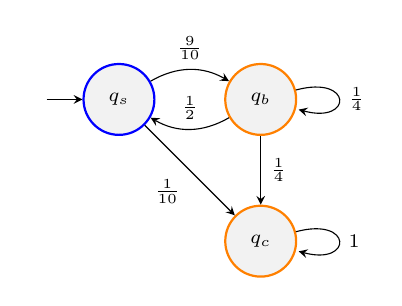
\begin{tikzpicture}[node distance=1.8cm,every node/.style={font=\scriptsize}]
            \node[state,initial, draw=blue] (qs) {$q_s$};
            \node[state, draw=orange] (qb) [right of=qs] {$q_b$};
            \node[state, draw=orange] (qc) [below of=qb] {$q_c$};

            \draw[->] (qs) edge[bend left] node[above] {$\frac{9}{10}$} (qb);
            \draw[->] (qs) edge node[below left] {$\frac{1}{10}$} (qc);
            \draw[->] (qb) edge[bend left] node[above] {$\frac{1}{2}$} (qs);
            \draw[->] (qb) edge[loop right] node {$\frac{1}{4}$} ();
            \draw[->] (qb) edge node[right] {$\frac{1}{4}$} (qc);
            \draw[->] (qc) edge[loop right] node {$1$} ();
        \end{tikzpicture}
        \caption{Example HMM, where the orange states $q_b$ and $q_c$ have the observation $bend$ and the blue state $q_s$ has the observation $straight$.}
        \label{fig:centralhmm}
    \end{subfigure}
    \hfill
    \begin{subfigure}{0.45\textwidth}
        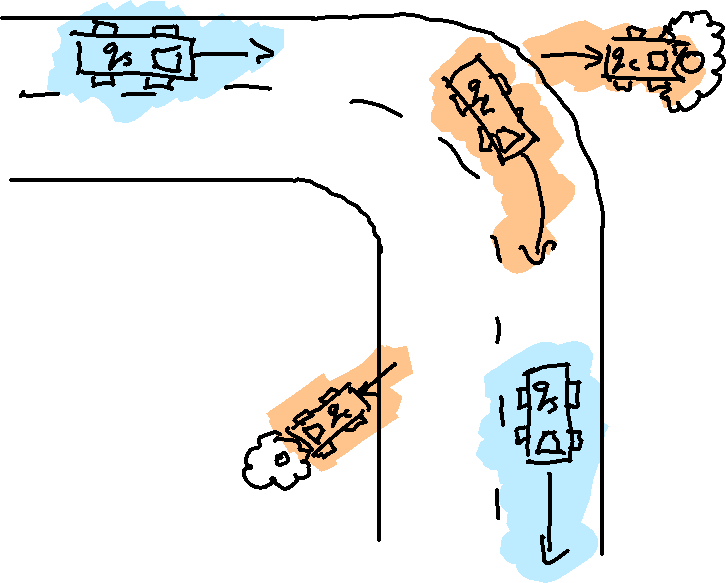
\includegraphics[width=\textwidth]{images/rM drawing 2024-12-18-15.01.17}
        \caption{Situation modeled by \cref{fig:centralhmm}. The cars are labeled by the state in the HMM they represent.}
    \end{subfigure}
    \begin{subfigure}{\textwidth}
        \center
        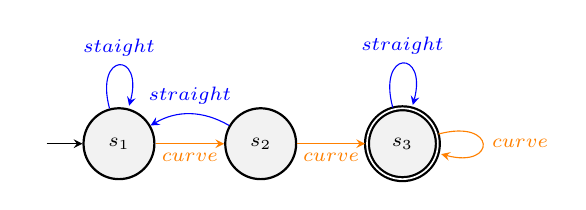
\begin{tikzpicture}[node distance=1.8cm,every node/.style={font=\scriptsize}]
            \node[state,initial] (q0) {$s_1$};
            \node[state] (q1) [right of=q0] {$s_2$};
            \node[state, accepting] (q2) [right of=q1] {$s_3$};

            \draw[->] (q0) edge[loop above, blue] node {$staight$} ();
            \draw[->] (q0) edge[orange] node[below] {$curve$} (q1);
            \draw[->] (q1) edge[blue, bend right] node[above] {$straight$} (q0);
            \draw[->] (q1) edge[orange] node[below] {$curve$} (q2);
            \draw[->] (q2) edge[orange, loop right] node {$curve$} ();
            \draw[->] (q2) edge[blue, loop above] node {$straight$} ();
        \end{tikzpicture}
        \caption{An example monitor for the HMM in \cref{fig:centralhmm}, which raises an alarm as soon as two steps in a curve have been observed.}
        \label{fig:centralmon}
    \end{subfigure}
    \caption{Central example to the paper}
    \label{fig:centralexample}
\end{figure}

\section{Monitor verification}
\label{sec:monver}
In this section we will discuss our solution to the monitor verification problem. We focuss on the no missed alarms problem, and adapt our solution to the no false alarms problem in \cref{ssec:nfa}.
We start by translating the problem to the Conditional trace probability (CTP) problem in \cref{ssec:ctp}, by incorporating the monitor in the HMM. Next, in \cref{ssec:polsyn}, we reduce the CTP problem to a consisitent policy synthesis problem for MDPs. Lastly, we show how to solve this consistent policy synthesis problem using PAYNT\cite{andriushchenkoPAYNTToolInductive2021} in \cref{ssec:paynt}.

\subsection{CTP problem}\label{ssec:ctp}
We will solve the Monitor verification problem by looking at the simpler \emph{Conditional trace probability} (CTP) problem. We will show a reduction from the Co-Monitor Verification Problem to CTP.
\begin{definition}[CTP Decision Problem]
    Given an HMM $\mc$ with colors $C$, a unary encoded horizon $H$, a set of goal states $G$, and a threshold $\lambda \in (0,1]$, is there a trace $\tau \in C^{H}$ such that $\sum_{\pi\in\Pi^\mc_H}\Prob^\mc(\pi_\downarrow \in G \mid \tau) \cdot r(\pi_\downarrow) \geq \lambda$.
\end{definition}
As we will be shown in \cref{sec:compl} the CTP problem is NP-complete.

The CTP problem differs from the monitor verification problem in two important aspects. First, the CTP problem no longer considers the monitor and the risk. Second, instead of deciding all traces are below a threshold, we have to find a trace above a threshold. Finding a trace similar to the dual of the Monitor Verification Problem, the \emph{co-Monitor Verification Problem}.
\begin{definition}[co-Monitor Verification Problem]
    Given a HMM $\mc$ with a state risk function $r: \Sts \to \RR_{\geq 0}$, a DAG monitor DFA $\dfa$ with as alphabet the observations of $\mc$, a risk thresholds $\lambda\in[0,\inf)$, and a horizon $h\in\NN^+$. Decide $R^{\max}_r(\overline{\dfa}) < \lambda$, where the \emph{weighted maximum risk function} $R_r^{\max}\colon DFA \to \RR_{\geq 0}$ is defined as
    \[
        R_r^{\max}(\dfa) := \underset{\tau\in\lang{\mc}\cap\lang{\dfa}}{\max} \sum_{\pi\in\Pi^h_\mc}\Prob(\pi \ |\ \tau) \cdot r(\pi_{\downarrow})
    \]
\end{definition}\todo{fix def}
Finding a trace in the co-MV problem disproves the MV problem for the same inputs.

\paragraph{Reduction to CTP}
\todo{Monitor needs to be complete}
In order to translate the co-MV problem to the CTP problem we combine the monitor in the HMM.
\todo{Maybe say complement of the monitor because missed alarms} In order to combine the monitor we make use of the Product Markov Chain construction from \citeauthor{baierPrinciplesModelChecking2008} \cite[def. 10.50]{baierPrinciplesModelChecking2008}. Our central example transformed into a CTP decision probelm can be found in \cref{fig:ctphmm}.

\begin{figure}[t]
    \centering
    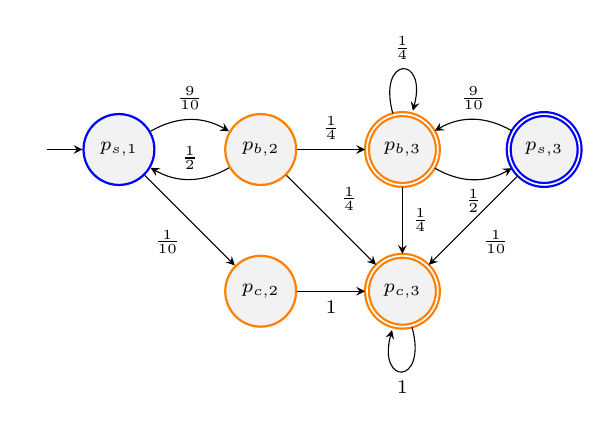
\begin{tikzpicture}[node distance=1.8cm,every node/.style={font=\scriptsize}]
        \node[state,initial, draw=blue] (qs1) {$p_{s,1}$};
        \node[state, draw=orange] (qb2) [right of=qs1] {$p_{b,2}$};
        \node[state, draw=orange] (qc2) [below of=qb2] {$p_{c,2}$};
        \node[state, draw=orange, accepting] (qb3) [right of=qb2] {$p_{b,3}$};
        \node[state, draw=orange, accepting] (qc3) [below of=qb3] {$p_{c,3}$};
        \node[state, draw=blue, accepting] (qs3) [right of=qb3] {$p_{s,3}$};

        \draw[->] (qs1) edge[bend left] node[above] {$\frac{9}{10}$} (qb2);
        \draw[->] (qs1) edge node[below left] {$\frac{1}{10}$} (qc2);

        \draw[->] (qb2) edge[bend left] node[above] {$\frac{1}{2}$} (qs1);
        \draw[->] (qb2) edge node[above] {$\frac{1}{4}$} (qb3);
        \draw[->] (qb2) edge node[above right] {$\frac{1}{4}$} (qc3);
        \draw[->] (qc2) edge node[below] {$1$} (qc3);

        \draw[->] (qc3) edge[loop below] node {$1$} ();
        \draw[->] (qb3) edge[loop above] node {$\frac{1}{4}$} ();
        \draw[->] (qb3) edge node[right] {$\frac{1}{4}$} (qc3);
        \draw[->] (qb3) edge[bend right] node[below] {$\frac{1}{2}$} (qs3);
        \draw[->] (qs3) edge[bend right] node[above] {$\frac{9}{10}$} (qb3);
        \draw[->] (qs3) edge node[below right] {$\frac{1}{10}$} (qc3);
    \end{tikzpicture}
    \caption{The central example HMM transformed into the CTP problem, using the Product Markov Chain construction \cite{baierPrinciplesModelChecking2008}. States are named with their HMM state, $\{s,b,c\}$ and their monitor state, $\{1,2,3\}$. States with the accepting label are marked as accepting states.}
    \label{fig:ctphmm}
\end{figure}

\subsection{Reduction to Policy Synthesis}\label{ssec:polsyn}
We will reduce the CTP problem into policy synthesis on Markov Decision Processes (MDPs).

\begin{definition}
    A Markov decision process is a tuple $\mdp=\left(\Sts, \Act, \ptrans, \init, \Aps, \lbl\right)$ where
    \begin{itemize}
        \item $\Sts$ is a countable set of states,
        \item $\Act$ is a set of actions,
        \item $\ptrans$ : $\Sts \times \Act \times \Sts \rightarrow[0,1]$ is the transition probability function such that for all states $s \in \Sts$ and actions $\alpha \in \Act$:

              \[
                  \sum_{s^{\prime} \in \Sts} \ptrans\left(s, \alpha, s^{\prime}\right) \in\{0,1\}
              \]

        \item $\init$ is the initial state,
        \item $\Aps$ is a set of atomic propositions, and
        \item $\lbl: S \rightarrow 2^{\Aps}$ is a labeling function.
    \end{itemize}

    From~\cite{baierPrinciplesModelChecking2008}
\end{definition}

In central idea behind reducing CTP to policy synthesis is letting a policy in the MDP coincide with a trace in the CTP HMM. To accomplish this we first unroll the CTP HMM over the horizon. Then, we let the actions of the MDP be the observations of the unrolled HMM, and thus, transform the model such that the policy can choose what observation to observe next. Then, we will add end transitions to all accepting states, such we have infinite paths corrensponding to finite traces. We outline these steps below.

\paragraph{Step 1}
The consruct the policy synthesis MDP $\mdp = (\Sts, C \cup \{end\}, P', \iota, \{\alarm, \safe\}, L)$
where $P'$ is definded as
\begin{align*}
    P'(s, c, q) :=
    \begin{cases}
        P^\mc(s,q)                                       & \text{if } \obsf(q) = c \\
        1 - \sum_{q'\in S\ |\ \obsf(q') = c} P^\mc(s,q') & \text{if } q = \iota    \\
        0                                                & \text{otherwise}
    \end{cases}
\end{align*}

\paragraph{Step 2}
We add two states to the MDP, an alarm state and a safe state. Both are sink states.
Every HMM state gets a new end transition:
\begin{align*}
    P'(s, end, alarm) :=
    \begin{cases}
        1 & \text{if } s \in G \\
        0 & \text{otherwise}
    \end{cases} \\
    P'(s, end, safe) :=
    \begin{cases}
        1 & \text{if } s \notin G \\
        0 & \text{otherwise}
    \end{cases}
\end{align*}
And we label the alarm and safe state using the alarm and safe labels respectively.


\begin{figure}
    \centering
    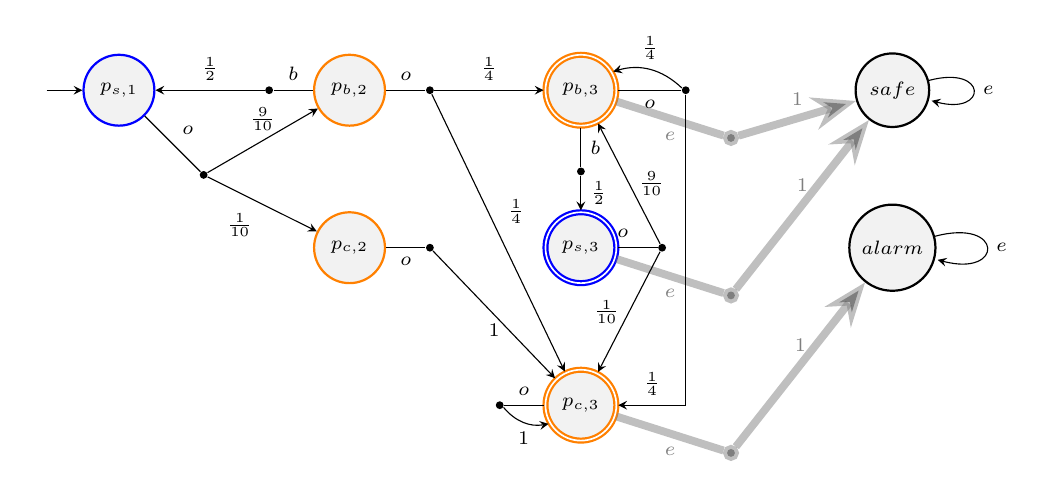
\begin{tikzpicture}[node distance=2cm,every node/.style={font=\scriptsize}]
        \node[state,initial, draw=blue] (qs1) {$p_{s,1}$};
        \node[action] (qs1o) [below right = 1cm of qs1] {};

        \node[state, draw=orange] (qb2) [right = 2cm of qs1] {$p_{b,2}$};
        \node[action] (qb2b) [left = .5cm of qb2] {};
        \node[action] (qb2o) [right = .5cm of qb2] {};

        \node[state, draw=orange] (qc2) [below of=qb2] {$p_{c,2}$};
        \node[action] (qc2o) [right = .5cm of qc2] {};

        \node[state, draw=orange, accepting] (qb3) [right = 2cm of qb2] {$p_{b,3}$};
        \node[action] (qb3b) [below = .5cm of qb3] {};
        \node[action] (qb3o) [right = .8cm of qb3] {};
        \node[action,risk] (qb3e) [below right = .2cm and 1.5cm of qb3] {};

        \node[state, draw=blue, accepting] (qs3) [below of=qb3] {$p_{s,3}$};
        \node[action] (qs3o) [right = .5cm of qs3] {};
        \node[action,risk] (qs3e) [below right = .2cm and 1.5cm of qs3] {};

        \node[state, draw=orange, accepting] (qc3) [below of=qs3] {$p_{c,3}$};
        \node[action] (qc3o) [left = .5cm of qc3] {};
        \node[action,risk] (qc3e) [below right = .2cm and 1.5cm of qc3] {};

        \node[state] (safe) [right= 3cm of qb3] {$safe$};
        \node[state] (alarm) [below of=safe] {$alarm$};

        \draw[risk, -] (qb3) edge node[below] {$e$} (qb3e);
        \draw[risk] (qb3e) edge node[above] {$1$} (safe);

        \draw[risk, -] (qs3) edge node[below] {$e$} (qs3e);
        \draw[risk] (qs3e) edge node[above] {$1$} (safe);

        \draw[risk, -] (qc3) edge node[below] {$e$} (qc3e);
        \draw[risk] (qc3e) edge node[above] {$1$} (alarm);

        \draw (qs1) edge node[above right] {$o$} (qs1o);
        \draw[->] (qs1o) edge node[above] {$\frac{9}{10}$} (qb2);
        \draw[->] (qs1o) edge node[below left] {$\frac{1}{10}$} (qc2);

        \draw (qb2) edge node[above] {$b$} (qb2b);
        \draw[->] (qb2b) edge node[above] {$\frac{1}{2}$} (qs1);
        \draw (qb2) edge node[above] {$o$} (qb2o);
        \draw[->] (qb2o) edge node[above] {$\frac{1}{4}$} (qb3);
        \draw[->] (qb2o) edge node[above right] {$\frac{1}{4}$} (qc3);

        \draw (qc2) edge node[below] {$o$} (qc2o);
        \draw[->] (qc2o) edge node[below] {$1$} (qc3);

        \draw (qc3) edge node[above] {$o$} (qc3o);
        \draw[->] (qc3o) edge[bend right] node[below] {$1$} (qc3);

        \draw (qb3) edge node[right] {$b$} (qb3b);
        \draw[->] (qb3b) edge node[right] {$\frac{1}{2}$} (qs3);
        \draw (qb3) edge node[below] {$o$} (qb3o);
        \draw[->] (qb3o) edge[bend right] node[above] {$\frac{1}{4}$} (qb3);
        \draw (qb3o) -- (qb3o|-qc3) edge[->] node[above] {$\frac{1}{4}$} (qc3);

        \draw (qs3) edge node[above left] {$o$} (qs3o);
        \draw[->] (qs3o) edge node[right] {$\frac{9}{10}$} (qb3);
        \draw[->] (qs3o) edge node[left] {$\frac{1}{10}$} (qc3);

        \draw (safe) edge[loop right] node {$e$} (safe);
        \draw (alarm) edge[loop right] node {$e$} (alarm);
    \end{tikzpicture}
    \caption{The central example transformed into an mdp to be used as the model in the MDP policy synthesis problem. Every state has an action which contains only transitions to states which had the observation related to that action.\todo[inline]{bad explanation}}
    \label{fig:mdpex}
\end{figure}

\subsubsection{Consistent schedulers}

\begin{definition}
    A \emph{consistent scheduler} is a scheduler which generates only the following traces
    \[\exists_{\tau\in\Sigma_{obs}}\ \forall_{\pi\in Paths(\sigma)}\ obs(\pi) = \cdots\iota\tau e^\star\]
    where $\iota$ is the observation of the initial state and $e$ is the observation of the $goal$ and $stop$ state.
\end{definition}
By model checking the created POMDP, we don't yet ensure that every scheduler is consistent, instead we only ensure semi-consistence.
\begin{definition}
    A semi-consistent scheduler $\sigma$ is a scheduler which has the following property \[\exists_{\tau\in\Sigma_{obs}}\ \forall_{\pi\in Paths(\sigma)}\ obs(\pi) = (\iota\tau^+)^\star\] where $\tau^+$ can be a different prefix of $\tau$ for every loop in $()^\star$.
\end{definition}

\subsection{Performing policy synthesis using memoryless policies}\label{ssec:paynt}

\subsection{Adapting to no false alarms}\label{ssec:nfa}

\section{Learning Monitors}

\section{Complexity}\label{sec:compl}

\begin{theorem}
    The monitor verification problem is ???-complete.
\end{theorem}

\subsubsection{Membership?}



\subsubsection{Hardness}
For hardness, we study the following simpler problem.
\textcolor{red}{CTP = Conditional trace probability. }

\begin{lemma}
    \label{lem:ctpdecnphard}
    The CTP Decision Problem is NP-hard.
\end{lemma}
\sebastian{What about the probability of a trace being zero?}

The result holds even for $\lambda = 1$ and acyclic HMMs. We illustrate the reduction from 3CNF.
Consider a 3CNF formula $\varphi = \bigwedge c_1 \dots c_m$ over $n$ variables $X$, with clause $c_j = \ell^1_j \lor \ell^2_j \lor \ell^3_j$ and each literal $\ell^i_j \in \{ x, \neg x \mid x \in X\}$. We transform this into a CTP instance with $\lambda = 1$ and an HMM with colours $C= \{ \#, \bot, \top \}$. We will create an HMM such that there is a trace with CPT $=1$ iff there is a satisfying assignment to the 3CNF formula.

Before we give a formal definition of the HMM, we give the following intuition, supported by Fig.~\ref{fig:hmmgadget}.
We represent assignments $\alpha\colon X \rightarrow \{0,1\}$ by traces through the HMM $\#\# \cdot \alpha(x_0) \cdot \# \cdot \alpha(x_1) \dots \cdot \#$. This trace matches with $m$ paths through the HMM, one for each clause. That is, the HMM randomly selects a clause with probability $\frac{1}{m}$ in the initial state and then evaluates this clause $c_j$ with respect to an assignment.
A path through a clause reads variable $x_i$ in state $s_{i,j}$ coloured with $\#$ and transitions to $s_{i,j}^\top$ and $s_{i,j}^\bot$, both with probability $0.5$. State $s_{i,j}^\top$ has colour $\top$, while $s_{i,j}^\bot$ has color $\bot$. Thus, the conditional probability to reach $s_{i,j}^\top$ is $\frac{1}{m}$ if $\alpha(x_i) = \top$ and $0$ otherwise.
Then, if the literal $x_i$ (or $\neg x_i$) occurs in clause $c_j$, we transition from $s_{i,j}^\top$ (or $s_{i,j}^\bot$, resp.) to $s_{i+1,j}'$, otherwise, we transition to $s_{i+1,j}$. The idea is that (conditionally) reaching state $s'_{i,j}$ (with positive probability) means that the partial assignment $\alpha(x_1),\dots,\alpha(x_i)$ satisfies clause $c_j$, while (conditionally) reaching $s_{i,j}$ (with positive probility) means that the clause is either unresolved or unsatisfied given the partial assignment.


\begin{figure}[t]
    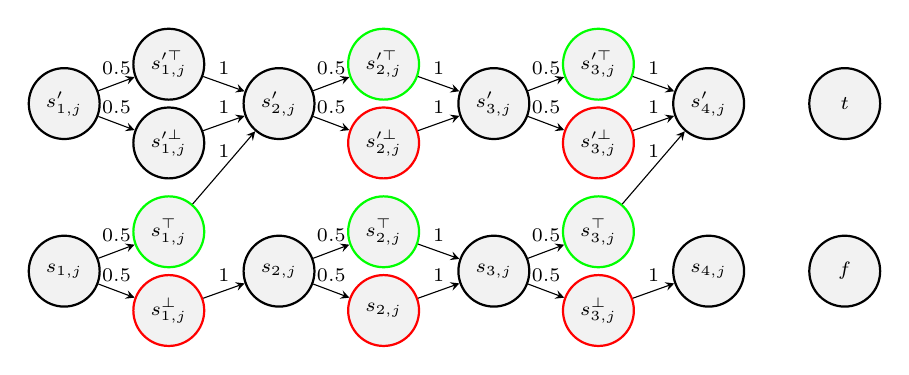
\begin{tikzpicture}[every node/.style={font=\scriptsize}]

        \node[state] (s1) {$s_{1,j}$};
        \node[state,right=0.4cm of s1,yshift=0.5cm,draw=green] (s1y) {$s_{1,j}^\top$};
        \node[state,right=0.4cm of s1,yshift=-0.5cm,draw=red] (s1n) {$s_{1,j}^\bot$};
        \node[state,above=1.2cm of s1,] (s1p) {$s'_{1,j}$};
        \node[state,right=0.4cm of s1p,yshift=0.5cm] (s1yp) {$s_{1,j}'^\top$};
        \node[state,right=0.4cm of s1p,yshift=-0.5cm] (s1np) {$s_{1,j}'^\bot$};
        \node[state,right=1.8cm of s1,] (s2) {$s_{2,j}$};
        \node[state,right=0.4cm of s2,yshift=0.5cm,draw=green] (s2y) {$s_{2,j}^\top$};
        \node[state,right=0.4cm of s2,yshift=-0.5cm,draw=red] (s2n) {$s_{2,j}$};
        \node[state,above=1.2cm of s2,] (s2p) {$s'_{2,j}$};
        \node[state,right=0.4cm of s2p,yshift=0.5cm,draw=green] (s2yp) {$s_{2,j}'^\top$};
        \node[state,right=0.4cm of s2p,yshift=-0.5cm,draw=red] (s2np) {$s_{2,j}'^\bot$};
        \node[state,right=1.8cm of s2,] (s3) {$s_{3,j}$};
        \node[state,right=0.4cm of s3,yshift=0.5cm,draw=green] (s3y) {$s_{3,j}^\top$};
        \node[state,right=0.4cm of s3,yshift=-0.5cm,draw=red] (s3n) {$s_{3,j}^\bot$};
        \node[state,above=1.2cm of s3,] (s3p) {$s'_{3,j}$};
        \node[state,right=0.4cm of s3p,yshift=0.5cm,draw=green] (s3yp) {$s_{3,j}'^\top$};
        \node[state,right=0.4cm of s3p,yshift=-0.5cm,draw=red] (s3np) {$s_{3,j}'^\bot$};
        \node[state,right=1.8cm of s3,] (s4) {$s_{4,j}$};
        \node[state,above=1.2cm of s4,] (s4p) {$s'_{4,j}$};
        \node[state,right=0.8cm of s4,] (f) {$f$};
        \node[state,above=1.2cm of f,] (t) {$t$};


        \draw[->] (s1) edge node[above] {$0.5$} (s1y);
        \draw[->] (s1) edge node[above] {$0.5$} (s1n);
        \draw[->] (s2) edge node[above] {$0.5$} (s2y);
        \draw[->] (s2) edge node[above] {$0.5$} (s2n);
        \draw[->] (s3) edge node[above] {$0.5$} (s3y);
        \draw[->] (s3) edge node[above] {$0.5$} (s3n);
        \draw[->] (s1p) edge node[above] {$0.5$} (s1yp);
        \draw[->] (s1p) edge node[above] {$0.5$} (s1np);
        \draw[->] (s2p) edge node[above] {$0.5$} (s2yp);
        \draw[->] (s2p) edge node[above] {$0.5$} (s2np);
        \draw[->] (s3p) edge node[above] {$0.5$} (s3yp);
        \draw[->] (s3p) edge node[above] {$0.5$} (s3np);

        \draw[->] (s1y) edge node[above] {$1$} (s2p);
        \draw[->] (s1n) edge node[above] {$1$} (s2);
        \draw[->] (s2y) edge node[above] {$1$} (s3);
        \draw[->] (s2n) edge node[above] {$1$} (s3);
        \draw[->] (s3y) edge node[above] {$1$} (s4p);
        \draw[->] (s3n) edge node[above] {$1$} (s4);
        \draw[->] (s1yp) edge node[above] {$1$} (s2p);
        \draw[->] (s1np) edge node[above] {$1$} (s2p);
        \draw[->] (s2yp) edge node[above] {$1$} (s3p);
        \draw[->] (s2np) edge node[above] {$1$} (s3p);
        \draw[->] (s3yp) edge node[above] {$1$} (s4p);
        \draw[->] (s3np) edge node[above] {$1$} (s4p);

    \end{tikzpicture}
    \caption{The main gadget for the reduction of Lemma~\ref{lem:ctpdecnphard}, demonstrated for the clause $x_1 \lor\neg x_3$ and variables $x_1, x_2, x_3$.}
    \label{fig:hmmgadget}
\end{figure}

We construct the following HMM $\mc = (\Sts, \ptrans, \init, \Aps, \lbl)$ and set $\lambda = 1$:
\begin{itemize}
    \item
          $\Sts = \{ s_{i,j}, s_{i,j}^\bot, s_{i,j}^\top,
              s_{i,j}', s_{i,j}'^\bot, s_{i,j}'^\top
              \mid i \in \{1, \dots, n+1 \},  j \in \{ 1, \dots, m \} \} \cup \{ s_\init \}$.
    \item $\ptrans$ is given such that for all $i \in \{1,\dots, n\}, j \in \{1, \dots, m\}$:
          \begin{itemize}
              \item  $\ptrans(s_\init,s_{1,j}) = \frac{1}{m}$,
              \item  $\ptrans(s_{i,j},s_{i,j}^\top) = \ptrans(s_{i,j},s_{i,j}^\bot) = \frac{1}{2}= \ptrans(s'_{i,j},s_{i,j}'^\top) = \ptrans(s_{i,j}',s_{i,j}'^
                        \bot)$,
              \item $\ptrans(s_{i,j}^\top,s'_{i+1,j}) = \indicator{x_i = \ell_j^k \text{ for some k}}$, $\ptrans(s_{i,j}^\top,s_{i+1,j}) = \indicator{x_i \neq \ell_j^k \text{ for all k}}$,
              \item $\ptrans(s_{i,j}^\bot,s'_{i+1,j}) = \indicator{\neg x_i = \ell_j^k \text{ for some k}}$, $\ptrans(s_{i,j}^\bot,s_{i+1,j}) = \indicator{\neg x_i \neq \ell_j^k \text{ for all k}}$
              \item $\ptrans(s'_{n+1,j}, t) = 1 = \ptrans(s_{n+1,j}, f)$
          \end{itemize}
    \item $c(s_{i,j}^\top) = (s_{i,j}'^\top) = \top$,
          $c(s_{i,j}^\bot) = (s_{i,j}'^\bot) = \bot$,
          $c(s_{i,j}) = c(s'_{i,j}) = \# = c(s_\init) = c(t) = c(f)$.
    \item

\end{itemize}

\begin{definition}[binary-CTP Decision Problem]
    Given an HMM $\mc$ with colors $C$, a binary encoded horizon $H$, and a threshold $\lambda \in (0,1]$, is there a trace $\tau \in C^{H}$ such that $\Prob^\mc(\lozenge G \mid \tau) \geq \lambda$.
\end{definition}

%\begin{lemma}
%\label{lem:ctpdecnphard}
%	The bin-CTP Decision Problem is in EXPTIME and NP-hard.
%\end{lemma}

\textcolor{red}{I have no clue how to show that is PSPACE hard... The PSPACE hardness would somehow have to use the long horizons.... I also dont believe it is important.}

\subsubsection{Approximability}

Approximating the verification of monitors is also hard, in the sense that it is hard to approximate the maximal risk that a monitor admits.

The maximal risk problem is an optimization problem
\begin{definition}[CTP Optimization Problem]

\end{definition}
\begin{lemma}
    The CTP Optimization Problem is APX-hard.
\end{lemma}
We show this by means of an L-reduction from MAX-3SAT, which is an inapproximable and APX-hard problem~\cite{}. The construction follows along the reduction for the NP-hardness.



\section{Experiments}
We build our tool in the python programming language on top of the model checker Storm \cite{henselProbabilisticModelChecker2022} and the POMDP model checker PAYNT \cite{andriushchenkoPAYNTToolInductive2021}. This tool includes both the \alg verifier algorithm and the learning algorithm employing \alg for equality queries.
\todo[inline]{TODO: Write further description of the tool.}

\paragraph{Benchmarks}
We evaluate both the \alg verifier and the learning algorithm. We evaluate the \alg verifier using the following questions:
\begin{description}
    \item[$\textbf{Q}_{VM}^1$] How does the runtime of \alg verifier depend on its parameters?
    \item[$\textbf{Q}_{VM}^2$] How much does the \alg verification depend on PAYNT?
    \item[$\textbf{Q}_{VM}^3$] Which PAYNT strategy is the most efficient in the \alg benchmarks? \todo{Maybe not a full question?}
\end{description}
We also evaluate the learning algorithm by looking at the following questions:
\begin{description}
    \item[$\textbf{Q}_{L}^1$] Does \alg learning guarantee a better bound then learning using a sampling EQ?
    \item[$\textbf{Q}_{L}^2$] How do the \alg learning monitors and sampling learning monitors compare in size?
    \item[$\textbf{Q}_{L}^3$] Do monitors learned without a horizon limit in MQ generalize to outside the horizon?\todo{Again, maybe less relevant?}
\end{description}

\section{Related}
LTLf

\section{Conclusion}

\printbibliography{}

\appendix

\section{Alternative formulations of the problem}
Instead of giving a specification DFA, we could instead give a TL specification~\cite{lichtensteinGlory1985} which is evaluated for every state. Since TL has both future and past operators both now reachability, $\diamond\hspace{-.9em}- l$, and soon reachability, $\bigcirc^n \diamond\hspace{-.9em}- l$, for a label $l$ can be expressed. While using a specification DFA can only express now reachability.

The only impact this reformulation of the problem would have is in step 1. Here, instead of taking the product MC, we check if the above described TL formula has a probability above a certain threshold. If that is the case we mark it with the $\circledcirc_\dfa$ label. This MC is then used for the subsequent steps.

\section{Reformulation with monitors}

\subsection{Benchmarks}


\section{Problem Statements}
We have two problems we want to solve. The no false alarms problem and the no missed alarms problem. They have slightly different problem statements and therefore also slightly different solutions.

\subsection{No false alarms}
All traces $\tau$ from the MC which are in the monitor have at least a probability $p\in I$ of reaching the good state.

\begin{definition}
    Given a Markov chain $\mc=\left(\Sts, \ptrans, \init, \Aps, \lbl\right)$ with observations in the set of colors $\Colors$, a specification DFA $\dfa=\left(\StsD_{\dfa}, 2^\Aps, \trans_{\dfa}, \init_{\dfa}, \final_{\dfa}\right)$, $\Aps$, and a DAG monitor DFA $\dfaB=\left(\StsD_{\dfaB}, C, \trans_{\dfaB}, \init_{\dfaB}, \final_{\dfaB}\right)$.
    For all traces $\tau$ from the MC and in the monitor, the probability of $\pi\in\lang{\dfa}$ given that $\pi$ conforms to $\tau$ is in a given interval $I$ \[\underset{\tau\in\lang{\mc}\cap\lang{\dfaB}}{\inter^I} \Prob^\mc(\pi\in\lang{\dfa}\ |\ \pi\in \Cyl(\Paths(\tau)))\]
\end{definition}

\subsection{No missed alarms}
All traces $\tau$ which reach the good state with probability $p > t$, are in the monitor. By taking the contrapositive, we can instead show that all traces $\tau$ which are not in the monitor reach the good state with probability $p \leq t$.

\begin{definition}
    Given a Markov chain $\mc=\left(\Sts, \ptrans, \init, \Aps, \lbl\right)$ with observations in the set of colors $\Colors$, a specification DFA $\dfa=\left(\StsD_{\dfa}, 2^\Aps, \trans_{\dfa}, \init_{\dfa}, \final_{\dfa}\right)$, $\Aps$, and a DAG monitor DFA $\dfaB=\left(\StsD_{\dfaB}, C, \trans_{\dfaB}, \init_{\dfaB}, \final_{\dfaB}\right)$.
    For all traces $\tau$ from the MC and not in the monitor, the probability of $\pi\in\lang{\dfa}$ given that $\pi$ conforms to $\tau$ is in a given interval $I$ \[\underset{\tau\in\lang{\mc}\cap\overline{\lang{\dfaB}}}{\inter^I} \Prob^\mc(\pi\in\lang{\dfa}\ |\ \pi\in \Cyl(\Paths(\tau)))\]
\end{definition}

\section{Outline}
See \cref{fig:outline} for an outline of the algorithm.

\begin{figure}[h]
    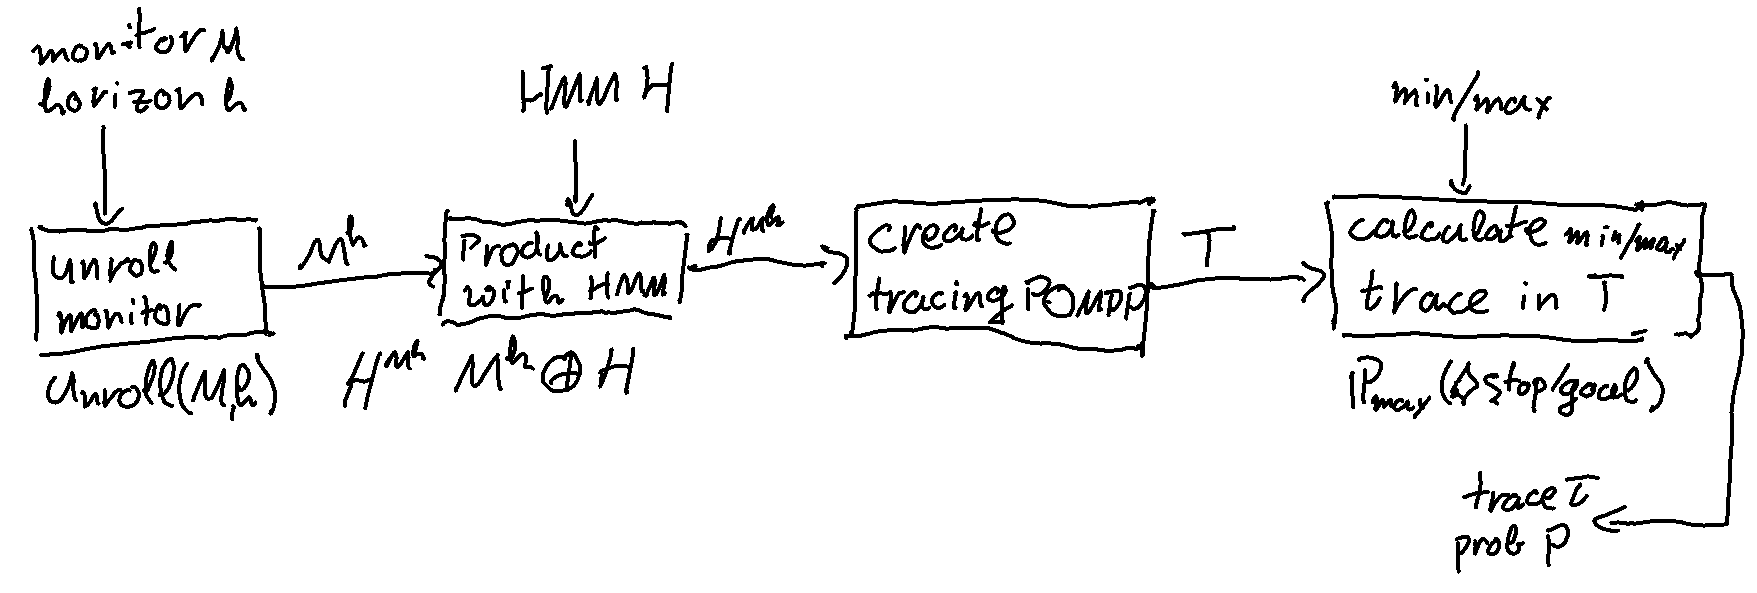
\includegraphics[width=\textwidth]{images/rM drawing 2024-11-28-13.42.46.png}
    \caption{Outline of the algorithm.}
    \label{fig:outline}
\end{figure}

\section{Algorithm}
Our algorithm will proceed in four steps. First, we take the MC product~\cite{baierPrinciplesModelChecking2008} of the MC $\mc$ and the specification $\dfa$. Then, we will combine the product MC with the monitor into an MDP. Next we will add end transitions to this MDP for all states that are accepted by the underlying monitor. Lastly, we use Paynt~\cite{andriushchenkoPAYNTToolInductive2021} to model check the created MDP.

\subsection{Applying the specification to the MC}
We take the MC product as defined by \citeauthor{baierPrinciplesModelChecking2008}~\cite{baierPrinciplesModelChecking2008} to create the product MC $\mc \oplus \dfa$.

\paragraph{Intuition}
The created product MC is the original MC, but every good state is labeled.

\subsection{Constructing the product MDP}
To create the MDP, we first create its states. The states are the product of the states of the product MC and the monitor. These are denoted as $\langle s, q_\dfaB\rangle$ for $s \in \Sts_{\mc \oplus \dfa}$, and $q_\dfaB \in \StsD_\dfaB$. As actions in the product MDP we take the observations $\Colors$ of the MC $\mc$.

The transitions in the MDP are defined here in two steps. First we create a not-yet-normalized transition function $P'$ on the states in the MDP. Next, we normalize the transition function by creating redirecting all remaining probability mass of an action in a state towards the initial state in $P''$.
\begin{align*}
    \large P'(\langle s, q\rangle , c, \langle s', q'\rangle) =  & \begin{cases}P(s, s') & \text{if } obs(s') = c \land q' = \delta(q, c)\\ 0 & \text{otherwise}\end{cases}                                                                                                                                              \\
    \large P''(\langle s, q\rangle , c, \langle s', q'\rangle) = & \begin{cases}1 - \sum_{s''\in S}\sum_{q''\in Q}P'(\langle s, q\rangle , c, \langle s'', q''\rangle) & \text{if } s' = \iota_{\mc\oplus\dfa} \land q' = \iota_\dfaB\\ P'(\langle s, q\rangle , c, \langle s', q'\rangle) & \text{otherwise}\end{cases}
\end{align*}

Lastly, the atomic propositions are $\{\circledcirc_\dfa, \circledcirc_\dfaB\}$, where accepting states in the product MC are labeled by $\circledcirc_\dfa$ and accepting states in the monitor are labeled by $\circledcirc_\dfaB$.

\paragraph{Intuition}
The created MDP can be seen as the original product MC $\mc\oplus\dfa$, where we can choose which observation to observe, but only if the monitor contains the transition labeled by the observation.

\subsection{Adding end transitions}
We add two new states to the MDP, the $goal$ and $stop$ states, each only having a self loop. Next, we will add an $end$ action to every state with the label $\circledcirc_\dfaB$. If the state also contains the $\circledcirc_\dfa$ label, we direct the $end$ action to the $goal$ state, otherwise we direct the $end$ action to the stop state.

\paragraph{Intuition}
Since we are talking about finite traces in the monitor, we need to give the MDP a way to end a path. This is done by taking the $end$ action. If we take the end action in a good state of the product MDP, we reach the $goal$ state, if it was a bad state, then we reach the $stop$ state.

\subsection{Model checking using Paynt}
We create a POMDP which will be model checked by Paynt~\cite{andriushchenkoPAYNTToolInductive2021} for reachability of the goal state. The observations in this POMDP are the states of the monitor. Using this POMDP we calculate \[\mathbb{P}_{\max}[\diamond goal]\] to find the maximum probability and \[1-\mathbb{P}_{\max}[\diamond stop]\] to find the minimum probability. Finally, we can verify this upper and lower bound with the interval $I$.

\paragraph{Intuition}
In order to find the traces in the monitor which give the maximum and minimum probability of reaching a good state, we associate a trace $\tau$ with a scheduler $\sigma_\tau$ in an MDP. Such a scheduler is called consistent.
\begin{definition}
    A \emph{consistent scheduler} is a scheduler which generates only one trace
    \[\exists_{\tau\in\Sigma_{obs}}\ \forall_{\pi\in Paths(\sigma)}\ obs(\pi) = \cdots\iota\tau e^\star\]
    where $\iota$ is the observation of the initial state and $e$ is the observation of the $goal$ and $stop$ state.
\end{definition}
By model checking the created POMDP, we don't yet ensure that every scheduler is consistent, instead we only ensure semi-consistence.
\begin{definition}
    A semi-consistent scheduler $\sigma$ is a scheduler which has the following property \[\exists_{\tau\in\Sigma_{obs}}\ \forall_{\pi\in Paths(\sigma)}\ obs(\pi) = (\iota\tau^+)^\star\] where $\tau^+$ can be a different prefix of $\tau$ for every loop in $()^\star$.
\end{definition}
Thus, a semi-consistent scheduler does not have to take and end action. However, by maximizing the probability of reaching either the $goal$ or $stop$ state, we ensure that if the $end$ action can be taken, it will be taken. And if a path takes the $end$ action, almost surely any other path will also take the $end$ action at some point. This property ensures that when maximizing semi-consistent schedulers we will always get a consistent scheduler, and thus a single trace.

\printbibliography{}

\end{document}